% FG WM Workshop @ KI 2026 — Full Paper
% CEUR-WS format, 6–12 pages
\documentclass[hf]{ceurart}

\usepackage{booktabs}
\usepackage{microtype}
\usepackage{amsmath}
\usepackage{pifont}
\usepackage{tikz}
\usepackage{pgfplots}
\usepgfplotslibrary{polar}
\pgfplotsset{compat=1.18}
\usetikzlibrary{shapes.geometric,arrows.meta,positioning,calc}

% Excalidraw-style palette
\definecolor{exgray}{HTML}{868e96}
\definecolor{exblue}{HTML}{4263eb}
\definecolor{exgreen}{HTML}{2b8a3e}
\definecolor{exorange}{HTML}{e67700}
\definecolor{exviolet}{HTML}{7048e8}

\begin{document}

\copyrightyear{2026}
\copyrightclause{Copyright for this paper by its authors.
  Use permitted under Creative Commons License Attribution 4.0
  International (CC BY 4.0).}

\conference{FGWM 2026: Workshop of the GI Special Interest Group on
  Knowledge Management, August 11--12, 2026, Bremen, Germany}

\title{Graph-Structured Memory for Cognitive Agents:\\
  From Knowledge Graphs to Non-Euclidean Geometry}

\author{Michael Banf}[email=michael.banf@perelyn.com]
\author{Johannes Kuhn}
\author{Slawomir Garcarz}
\author{Liliya Imasheva}
\author{Dominik Filipiak}
\author{Marc Stiller}
\author{Christian Mader}
\author{Gustaw Kalek}
\author{Maximilian Schattauer}
\author{Anton Steuer}
\author{Gzregorz Luczyna}
\author{Konstantin Gärtner}
\author{Emily Rasenecker}
\author{Max Becker}
\author{Sebastian Fetz}

\address{Perelyn GmbH, Munich, Germany}

\begin{abstract}
Large language model based agents require persistent memory that
spans sessions, tracks temporal evolution, and supports multi-hop
reasoning. As context windows grow, the na\"{\i}ve strategy is to
compress all prior interaction into the prompt, however compression
discards relational structure. Graph-structured memory offers a
fundamentally different approach: store knowledge in a graph and
retrieve selectively. Yet current systems embed these graphs
exclusively in Euclidean space, incurring distortion on the
hierarchical, tree-like structures inherent to agent memory.
We survey research papers between 2023 and 2026, identifying six
architectural patterns and a retrieval spectrum from training-free
graph algorithms to graph neural network message passing. We then analyze how
non-Euclidean geometric techniques, such as discrete Ricci curvature for
diagnosing retrieval bottlenecks, hyperbolic embeddings for
hierarchy-preserving retrieval, Lie group manifolds for temporal
knowledge graph fusion, and mixed-curvature product spaces, are
already proven in retrieval and KG reasoning, with significant gains
over Euclidean baselines. We argue that since agent memory is fundamentally
retrieval over a persistent knowledge graph, these techniques are
directly applicable as foundational layers, but integrating them into
cross-session memory architectures is the defining open challenge.
\end{abstract}

\begin{keywords}
  Knowledge Graphs \sep
  Agent Memory \sep
  Non-Euclidean Geometry \sep
  Hyperbolic Embeddings \sep
  Temporal Knowledge Graphs \sep
  LLM Agents
\end{keywords}

\maketitle


%%% ==================================================================
\section{Introduction}
%%% ==================================================================

The dominant memory pattern for Large Language Model (LLM) agents is stateless: each session
begins from scratch. When persistence is added, it typically takes one
of two forms: i)~flat extraction, i.e. triplet stores, key-value memories,
or embedding-indexed chunks~\cite{mem0_2025,packer2023}; or
ii)~brute-force compression of all prior interaction into the context
window, which grows ever larger but still cannot preserve relational
structure. Both handle factual recall but fail systematically on
temporal reasoning, multi-hop inference, and knowledge evolution.
Flat paradigms---vector stores, key-value extraction, and even
the emerging LLM Wiki pattern~\cite{karpathyllmwiki2025}---lack
native support for multi-hop traversal, temporal ordering, causal
structure, and hierarchical consolidation; graph-based architectures
provide all of these by construction.
Benchmark evidence quantifies the deficit:
LoCoMo-Plus~\cite{gurawaliya2026} reports cognitive accuracy below 25\%
across Mem0, Letta, and Zep, with a 35--45\,pp drop from
factual to cognitive tasks. MemoryAgentBench~\cite{memoryagentbench2026}
finds all methods below 7\% on multi-hop conflict resolution, while multi-strategy systems combining graph traversal with vector search
achieve 91.4\% retrieval accuracy versus 49.0\% for extraction-based
systems~\cite{vectorize2026}. Graph-structured memory offers a fundamentally different
strategy: instead of compressing everything into the context window,
store knowledge in a graph and retrieve selectively. Knowledge graphs (KG)
ground entities and relations while temporal KGs add validity intervals;
hierarchical event graphs capture episodic consolidation. The core
challenge then shifts from \emph{what to discard} to \emph{how to
find the right subgraph}, i.e. a retrieval problem where graph topology is
a first-class signal.
Here we survey the current state of the art graph-based agent memory systems between 2023--2026~\cite{graphmemsurvey2026, memagents2026}, 
with three significant findings standing out: i)~entity-relation KGs account for 60\% of surveyed graph-memory papers;
non-KG structures remain rare; ii)~57\% implement no temporal mechanism, constituting a field-wide deficit; and iii)~retrieval is overwhelmingly training-free, i.e. graph algorithms and
multi-strategy heuristics power every production system, while only a tiny fraction of surveyed research work applies graph neural networks (GNN) message passing.

Figure~\ref{fig:progression} illustrates the structural progression
from flat memory to geometric representations. This paper contributes:
(1)~a taxonomy of graph-based agent memory patterns including temporal
grounding;
(2)~a retrieval spectrum with a model-size equalizer analysis;
(3)~an analysis of non-Euclidean geometric techniques and their
application to agent memory challenges; and
(4)~a research agenda.

\begin{figure}[t]
\centering
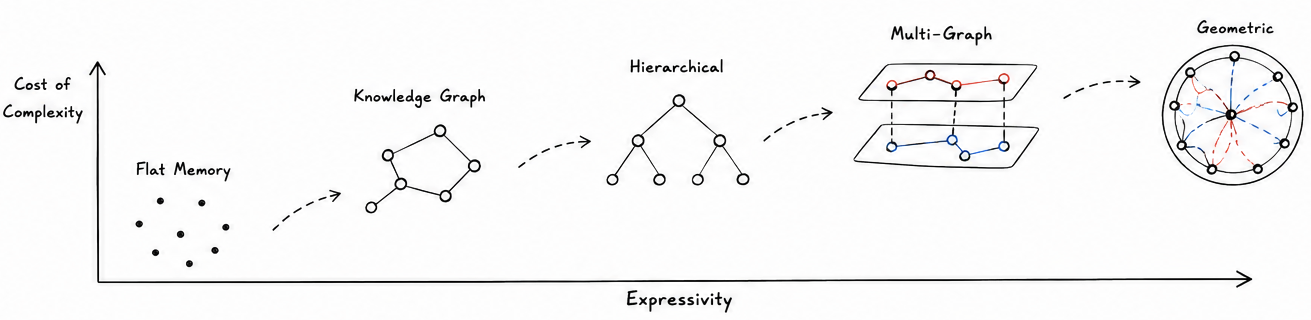
\includegraphics[width=\textwidth]{overview.png}
\caption{Structural progression of agent memory representations. Each
  level adds expressivity at the cost of complexity. Current production
  systems operate at the knowledge graph and hierarchical levels, while geometric
  representations remain a largely unexplored frontier.}
\label{fig:progression}
\end{figure}





%%% ==================================================================
\section{Taxonomy of Graph-Based Agent Memory}
\label{sec:taxonomy}
%%% ==================================================================

From our classification we identify four established architectural patterns, two emerging
ones, and a cross-cutting temporal dimension (Table~\ref{tab:systems}).
%
The most prevalent pattern is the \emph{entity-relation knowledge graph},
representing memory as typed $(subject, relation, object)$ triples.
CraniMem~\cite{cranimem2026} combines a bounded FIFO episodic buffer
with an entity-relation KG. UltRAG~\cite{ultrag2026} queries
large-scale KGs via a pre-trained GNN foundation
model. AriGraph~\cite{arigraph2025} integrates episodic and semantic memory
within a single KG. GraphRAG~\cite{graphrag2024} clusters via Leiden
into hierarchical community summaries. Entity-relation KGs excel at
factual memory but are limited to binary relations.

The \emph{Hierarchical event graphs} pattern addresses this by maintaining episodic
and semantic layers with cross-layer edges. GAM~\cite{gam2026} combines a Topic Associative Network with Event
Progression Graphs. MemFly~\cite{memfly2026} implements a three-layer
hierarchy via the Information Bottleneck principle. \cite{ctc2026} introduces Cue-Tag-Content heterogeneous graphs.
MemGraphRAG~\cite{memgraphrag2026} organizes memory into three
layers (ontology schemas, entity-relation facts, source passages)
with multi-agent self-adjudication, i.e. a conflict detection agent
identifies inconsistencies and a resolution agent adjudicates via
provenance evidence, demonstrating that filtering
low-frequency triples actually improves accuracy on
multi-hop Question Answering.


\begin{table*}[t!]
\caption{Comparison of graph-based agent memory systems.
  Temporal: \ding{51}\,=\,deep mechanism, $\triangle$\,=\,timestamps/decay,
  ---\,=\,none. Retrieval: GA\,=\,graph algorithms,
  MS\,=\,multi-strategy, RL\,=\,reinforcement learning,
  GNN\,=\,message passing, AB\,=\,agent-based.}
\label{tab:systems}
\centering\scriptsize
\begin{tabular*}{\textwidth}{@{\extracolsep{\fill}}llcclrl@{}}
\toprule
\textbf{System} & \textbf{Graph Type} & \textbf{Temp.} & \textbf{Retr.} & \textbf{Evolution} & \textbf{Best Score} & \textbf{Benchmark} \\
\midrule
\multicolumn{7}{@{}l}{\textit{Production \& multi-strategy systems}} \\
Zep/Graphiti & KG (bi-temporal) & \ding{51} & MS & Temporal invalidation & 94.8\% & Deep Mem.\ Retrieval \\
Hindsight & KG + vector & $\triangle$ & MS & --- & 91.4\% & LongMemEval \\
FalkorDB+Mem0 & KG (graph DB) & --- & MS & Dedup/merge & $<$140\,ms p99 & Production \\
\midrule
\multicolumn{7}{@{}l}{\textit{Hierarchical \& multi-graph architectures}} \\
GAM & Hierarchical (2-layer) & $\triangle$ & GA & State-based consol. & 40.00 F1 & LoCoMo (7B) \\
MAGMA & Multi-graph (4 types) & \ding{51} & GA & Dual-stream consol. & 0.700 & LoCoMo Judge \\
MemFly & Hierarchical (3-layer) & --- & GA & IB clustering & 44.4 F1 & LoCoMo (GPT-4o) \\
MemGraphRAG & Hier.\ (3-layer) & --- & MS & Schema filter + adjud. & 59.25\% & Multi-hop QA \\
\midrule
\multicolumn{7}{@{}l}{\textit{Entity-relation KG systems}} \\
Mem0 & KG (entity-relation) & --- & GA & Dedup/merge & 28.86 F1 & LoCoMo (7B) \\
HippoRAG & KG (open) & --- & GA & --- & +3--10 F1 & Multi-hop QA \\
CraniMem & KG (gated buffer) & --- & GA & Replay consol. & $-$0.011 F1 & HotpotQA noise \\
\midrule
\multicolumn{7}{@{}l}{\textit{Temporal-aware systems}} \\
RecallM & KG (temporal window) & \ding{51} & GA & Context revision & 4$\times$ vs Vec & Temporal QA \\
MemoTime & KG (Tree of Time) & \ding{51} & GA & Temporal monoton. & --- & Temporal reason. \\
TReMu & KG (neuro-symbolic) & \ding{51} & GA & Code-gen dates & --- & Multi-session \\
\midrule
\multicolumn{7}{@{}l}{\textit{RL \& learned retrieval systems}} \\
TGM & Procedural (3-layer) & --- & RL & REINFORCE weights & 0.426 EM & HotpotQA (4B) \\
Memory-R1 & KG & --- & RL & RL operations & --- & Memory via RL \\
\midrule
\multicolumn{7}{@{}l}{\textit{GNN \& higher-order systems}} \\
LP-RAG & Bipartite & --- & GNN & --- & +2.8\% EM & Multi-hop QA \\
MemoGraph & KG + RGCN & --- & GNN & --- & 86.9\% & MATH (7B) \\
HyperMem & Hypergraph (3-level) & --- & GA & --- & --- & --- \\
\midrule
\multicolumn{7}{@{}l}{\textit{Multi-agent \& procedural systems}} \\
Collabor Mem. & KG (shared) & --- & AB & Access control & --- & Multi-agent \\
PRAXIS & State-action tuples & --- & GA & Real-time learn. & 44.1\% & REAL (web) \\
SkillRL & Hier.\ SkillBank & --- & RL & Recursive evol. & +14\% & ALFWorld \\
SimpleMem & Multi-view index & --- & MS & Sem.\ compression & +26.4\% F1 & LoCoMo \\
\bottomrule
\end{tabular*}
\end{table*}



\emph{Bipartite and associative graphs} take a lighter approach.
For example, LP-RAG~\cite{lprag2026} constructs a bipartite chunk-query graph
with mutual $k$-NN edges (retrieval via GNN link prediction
outperforms embedding similarity by 1.6--2.8\% EM), while
AssoMem~\cite{assomem2025} anchors dialogue to automatically
extracted clues, i.e. minimal overhead, but limited representational
power.

At the other extreme, \emph{multi-graph composites} maintain several
orthogonal views simultaneously. MAGMA~\cite{magma2026} connects event-nodes via four edge types
(temporal, causal, semantic, entity) with dual-stream fast/slow
consolidation. TM2RAG~\cite{tm2rag2026} extends this with five graphs unified
through a meta graph.

Two emerging patterns push beyond pairwise relations.
\emph{Hypergraph memory} systems, such as HyperGraphRAG~\cite{hypergraphrag2025},
HyperMem~\cite{hypermem2026}, HGMem~\cite{hgmem2025}, use hyperedges
for $n$-ary facts and multi-step reasoning chains, though all treat
the hypergraph as a data structure without higher-order message
passing. \emph{Procedural strategy graphs} encode agent trajectories directly:
Trainable Graph Memory (TGM)~\cite{trainablegraph2025} represents
trajectories as a heterogeneous DAG optimized via REINFORCE, where
the trained Qwen3-4B outperforms baseline Qwen3-8B, i.e. procedural graph memory substituting for model scale. PRAXIS~\cite{praxis2026} implements
procedural memory for web agents. SkillRL~\cite{skillrl2026} builds
a hierarchical SkillBank.

Cutting across all patterns is the question of \emph{temporal
grounding}. Despite being the central promise of graph-based memory,
57\% of surveyed papers implement no temporal mechanism and only 20\% go
beyond timestamps. Graphiti/Zep~\cite{rasmussen2025} provides the
most complete solution via a bi-temporal model distinguishing
event time from ingestion time, where every edge
carries validity intervals. RecallM~\cite{recallm2023} uses temporal windows with
Hebbian-inspired relation strength for a more effective belief
updating than vector databases. MemoTime~\cite{memotime2025} organizes temporal reasoning into
time trees, while TReMu~\cite{tremu2025}, similarly to Graphiti/Zep, decouples mention time
from event time. Biologically inspired mechanisms offer implicit temporal grounding. For example,
Mnemosyne~\cite{mnemosyne2025} applies exponential decay with spreading activation. MIRROR~\cite{mirror2026} validates fast
encoding plus slow consolidation. MARTA~\cite{marta2026} uses predictive entropy to arbitrate
retrieval. However, a staleness gap persists, i.e. no system tracks when abstracted
semantic knowledge becomes outdated.

%%% ==================================================================
\section{From Graph Algorithms to Learned Retrieval}
\label{sec:retrieval}
%%% ==================================================================

Memory retrieval over graphs spans a spectrum from training-free
algorithms to fully learned neural approaches. The dominant approaches require no training. For example
HippoRAG~\cite{hipporag2024} implements Personalized PageRank as a
neurobiologically inspired pattern-completion mechanism.
GraphRAG~\cite{graphrag2024} and MemFly use Leiden for community
detection. GAM applies exponential recency decay. These algorithms
work on any graph at 10--150\,ms, explaining why every deployed
system adopts them. Production systems go further by combining multiple pathways. E.g.
Hindsight~\cite{hindsight2025} executes semantic search, BM25, graph
traversal, and temporal filtering simultaneously, fusing via
cross-encoder. SimpleMem~\cite{simplemem2026} achieves improvement over
Mem0 while reducing tokens via three-stage semantic
compression. Beyond heuristics, RL-based approaches learn to optimize different
aspects of graph memory, such as edge weights~\cite{trainablegraph2025}, memory operations~\cite{memoryr12025}, graph construction~\cite{memalpha2025}, and unified retrieval-reasoning~\cite{memsearcher2025}. D-RAG~\cite{drag2025} enables
joint retriever-generator optimization through Gumbel-Softmax subgraph sampling.
At the far end of the spectrum, only a tiny fraction of the surveyed systems apply GNN message
passing, for example LP-RAG~\cite{lprag2026} recasts retrieval as inductive link
prediction, MemoGraph~\cite{memograph2026} encodes evolving reasoning
graphs. The scarcity reflects fundamental tensions, i.e. cold start, no retrieval labels, graph
evolution outpacing retraining, and diminishing returns on factual
tasks where heuristics already achieve high accuracy.

A striking pattern across our corpus is that graph-structured
memory disproportionately benefits smaller models. GAM achieves +39\% F1 improvement over
Mem0 at 7B but only +7\% at GPT-4o, and on LongDialQA this ratio reaches
17 times improvement. The trained Qwen3-4B with graph memory
outperforms baseline Qwen3-8B showing that graph structure directly
substitutes for model scale. GNN-RAG~\cite{gnnrag2025} shows a
fine-tuned 7B model with graph retrieval matches GPT-4 on knowledge graph question answering tasks.

These results may be explained by four mechanisms: i)~context window relief via focused
subgraph retrieval; ii)~explicit structure offloading reasoning that
larger models derive implicitly; iii)~token efficiency (GNN-RAG's
reduction); and iv)~strategic compensation from
meta-cognitive priors in graph structure. Finally, graph memory must evolve as agents accumulate experience, i.e.
consolidation merges episodic observations into compressed semantic
representations, and
SkillRL~\cite{skillrl2026} achieves recursive skill co-evolution with
significant token compression versus raw trajectory storage.


%%% ==================================================================
\section{Geometric Representations for Agent Memory}
\label{sec:geometric}
%%% ==================================================================

All graph-based memory systems surveyed above embed their graphs in
flat Euclidean space. Yet recent work on graph neural networks,
knowledge graph embeddings, and topological deep
learning~\cite{tdlposition2024} shows that non-Euclidean
representations---hyperbolic embeddings, discrete Ricci curvature,
Lie group manifolds---can dramatically improve performance on
hierarchical and temporal data. Since graph-structured memory is
fundamentally a retrieval problem---finding the right subgraph at the
right time---these techniques are directly applicable as foundational
components of memory architectures.

Selective retrieval over a knowledge graph fails when the graph
topology itself creates bottlenecks. \emph{Discrete Ricci
curvature}~\cite{formanricci2017,topping2022} provides a per-edge
diagnostic for this: edges within tight clusters have positive
curvature, while edges bridging distant communities have negative
curvature. Negatively curved edges cause
\emph{over-squashing}~\cite{alon2021}---information from
exponentially many source nodes must squeeze through a single bridge
edge, causing multi-hop retrieval to suffer exponential signal
decay. This offers a structural explanation for the cognitive
accuracy ceiling below 25\%. Three concrete applications emerge:
i)~Forman-Ricci curvature provides a training-free, $O(|E|)$
diagnostic that flags edges where retrieval is likely to degrade;
ii)~Stochastic Discrete Ricci Flow (SDRF)~\cite{topping2022} offers
a principled geometric alternative to Leiden-based community
detection for hierarchical consolidation; and iii)~structural lifting
from graphs to
hypergraphs~\cite{banf2025helmholtz,hypergraphricci2024} can promote
bottleneck edges to hyperedges, restoring multi-hop connectivity.

Selective retrieval also fails when the embedding space itself cannot
separate what the graph distinguishes. As memory grows, Euclidean
spaces suffer from \emph{semantic collapse}: hierarchical structures
are compressed into a low-dimensional subspace because Euclidean
volume grows polynomially while tree-like knowledge branching grows
exponentially~\cite{nickel2017poincare}. Gao and
Metaxas~\cite{gao2026semanticshift} formalize this as semantic
shift---as diversity increases, pooled representations drift away
from every individual embedding. \emph{Hyperbolic space}, where
volume grows exponentially, provides a geometric remedy by naturally
separating hierarchy levels: abstract topics embed near the origin,
episodes in the middle ring, and specific facts near the boundary.
HyperbolicRAG~\cite{hyperbolicrag2025} fuses Euclidean and hyperbolic
rankings for hierarchy-aware retrieval.
HypRAG~\cite{hyprag2026} develops fully hyperbolic transformers in
the Lorentz model. HELM~\cite{helm2025} shows LLM token embeddings
already exhibit substantial negative Ricci curvature, suggesting that
LLM representations are naturally hyperbolic and motivating matching
the memory embedding space to the model's intrinsic geometry.
HyperVC~\cite{hypervc2022} applies variable-curvature hyperbolic
spaces to temporal KG snapshots. However,
HyperGCL~\cite{hypergcl2025} shows that naive contrastive learning in
hyperbolic space still causes dimensional collapse, meaning
collapse-aware objectives are required, such as HypRAG's Outward
Einstein Midpoint pooling operator. Since real memory graphs exhibit
topological heterogeneity---some regions are tree-like, others
cyclical or clique-dense---a single curvature may not suffice.
GraphMoRE~\cite{graphmore2025} addresses this with a mixture of
Riemannian experts that assigns spherical, hyperbolic, or Euclidean
geometry per node.

Cross-session memory further requires temporal reasoning: retrieving
not just what was stored but when, and how knowledge evolved. In
temporal KGs, entities, relations, and timestamps live in
fundamentally different spaces, making direct fusion difficult.
\emph{Lie groups} such as $SO(n)$ (rotation matrices) offer a
solution: their tangent space---the Lie algebra---is an ordinary
vector space, so projecting via the logarithmic map lets
heterogeneous factors be added, scaled, and processed by standard
neural network layers. Li et al.~\cite{tkgembed2025} apply this
using $SO(2)$ Givens rotations to unify temporal KG factor
embeddings. TeAST~\cite{teast2023} maps temporal relations onto
Archimedean spiral geometry.
TempHypE~\cite{temphype2025} unites Poincar\'{e} ball embeddings
with Neural ODEs for continuous-time evolution.
RicciKGE~\cite{riccikge2025} co-evolves Ricci flow with KG
embeddings, where curvature smooths bottleneck regions while updated
embeddings reshape curvature. At the foundation-model scale,
RiemannGFM~\cite{riemanngfm2025} learns cross-domain transferable
Riemannian graph representations, suggesting that zero-shot geometric
encoding of memory traces may become feasible without per-agent
supervised training.

These geometric techniques are already proven in retrieval and KG
reasoning. The open challenge is integrating them into persistent,
cross-session memory architectures with evolving graphs.

%%% ==================================================================
\section{Open Challenges and Conclusion}
\label{sec:agenda}
%%% ==================================================================

Graph-structured memory reframes the persistence problem. Instead of
compressing everything into the context window, store knowledge in a
graph and retrieve selectively. Our survey shows
this paradigm works with multi-strategy retrieval reaching top performances on
long memory evaluation benchmarks, and graph memory equalizing even small models to near-frontier
performance at significant lower cost. However, but several challenges
remain. Current systems vary widely in graph types, node/edge
semantics, and temporal models. Therefore, a unified ontology specifying how
entities, events, temporal intervals, and higher-order groupings
compose would enable interoperability and memory transplantation
across architectures~\cite{transplants2026}. Graph algorithms
dominate practice while GNN-based message passing remains limited to
a handful of systems. Hence, whether learned structural representations can
break the cognitive ceiling is an open
question. Collaborative memory is largely unexplored, yet the same relational
structure that enables rich retrieval also enables adversarial
injection~\cite{minja2026,collabormem2025,damcs2025}. Memory quality
deserves attention beyond downstream accuracy, i.e. diagnostic
analysis~\cite{diagnosebottleneck2026} reveals that retrieval
quality, not write-time sophistication, remains the primary bottleneck,
and filtering low-frequency schema triples actually improves accuracy. Scalability
is also a practical concern, with systems spanning wide latency
ranges, and at lifetime scale, approximate retrieval, compression, and
asynchronous processing~\cite{comem2026} become critical. Finally,
geometric retrieval techniques such as curvature diagnostics, hyperbolic
embeddings, mixed-curvature manifolds, and continuous-time
dynamics, are proven in retrieval and knowledge graph reasoning but await
systematic integration into persistent, cross-session memory
architectures. Addressing these challenges collectively would move
the field from isolated retrieval components toward truly unified
agent memory that is persistent, geometry-aware, and capable of the
structured recall that cognitive continuity demands.


%%% ==================================================================
\begin{thebibliography}{50}
%%% ==================================================================

\bibitem{memgraphrag2026}
Wu, C., et al.: MemGraphRAG: Memory-based Multi-Agent System for
Graph Retrieval-Augmented Generation. In: KDD 2026.
arXiv:2606.00610

\bibitem{mem0_2025}
Chhikara, P., et al.: Mem0: Building Production-Ready AI Agents with
Scalable Long-Term Memory. In: ECAI 2025

\bibitem{packer2023}
Packer, C., et al.: MemGPT: Towards LLMs as Operating Systems.
arXiv:2310.08560 (2023)

\bibitem{gurawaliya2026}
Gurawaliya, H., Nalenz, M., Ma, M.: Agentic Memory Realized: From
Stateless Models to Cognitive Continuity. appliedAI Initiative (2026)

\bibitem{memoryagentbench2026}
Hu, Y., et al.: MemoryAgentBench: Evaluating Memory in LLM Agents via
Incremental Multi-Turn Interactions. In: ICLR 2026

\bibitem{vectorize2026}
Vectorize: Best AI Agent Memory Systems---Architecture, Benchmarks,
and Trade-offs. Vectorize.io (2026)

\bibitem{graphmemsurvey2026}
Yang, C., et al.: Graph-based Agent Memory: Taxonomy, Techniques,
and Applications. arXiv:2602.05665 (2026)

\bibitem{memagents2026}
MemAgents: Memory for LLM-Based Agentic Systems. ICLR 2026 Workshop

\bibitem{hipporag2024}
Gutierrez, B.J., et al.: HippoRAG: Neurobiologically Inspired
Long-Term Memory for Large Language Models. In: NeurIPS 2024

\bibitem{rasmussen2025}
Rasmussen, P., et al.: Zep: A Temporal Knowledge Graph Architecture
for Agent Memory. arXiv:2501.13956 (2025)

\bibitem{hindsight2025}
Hindsight: Open-Source AI Memory System with Multi-Strategy Retrieval.
GitHub (2025)

\bibitem{graphrag2024}
Edge, D., et al.: From Local to Global: A Graph RAG Approach to
Query-Focused Summarization. arXiv:2404.16130 (2024)

\bibitem{cranimem2026}
CraniMem: Cranial-Inspired Gated and Bounded Memory for Agentic
Systems. In: MemAgents Workshop, ICLR 2026

\bibitem{ultrag2026}
UltRAG: A Universal Simple Scalable Recipe for Knowledge Graph RAG.
In: MemAgents Workshop, ICLR 2026

\bibitem{arigraph2025}
Anokhin, P., et al.: AriGraph: Learning Knowledge Graph World Models
with Episodic Memory for LLM Agents. In: IJCAI 2025

\bibitem{gam2026}
Wu, Z., et al.: GAM: Hierarchical Graph Memory for LLM-based
Agents. In: MemAgents Workshop, ICLR 2026

\bibitem{memfly2026}
MemFly: On-the-Fly Memory Optimization via Information Bottleneck.
In: MemAgents Workshop, ICLR 2026

\bibitem{ctc2026}
Memory is Reconstructed, Not Retrieved: Graph Memory for LLM Agents.
In: MemAgents Workshop, ICLR 2026

\bibitem{lprag2026}
LP-RAG: A Link Prediction-Based Framework for Retrieval-Augmented
Generation. In: MemAgents Workshop, ICLR 2026

\bibitem{assomem2025}
Zhang, K., et al.: AssoMem: Scalable Memory QA with Multi-Signal
Associative Retrieval. arXiv:2510.10397 (2025)

\bibitem{magma2026}
MAGMA: A Multi-Graph based Agentic Memory Architecture for AI
Agents. arXiv:2601.03236 (2026)

\bibitem{tm2rag2026}
Shibui, Y.: Organizing Documents with Temporal, Multimodal,
Multigraph Structures and Agentic RAG. (2026)

\bibitem{hypergraphrag2025}
HyperGraphRAG: Hypergraph-Driven Retrieval-Augmented Generation for
$n$-ary Relational Knowledge. In: NeurIPS 2025

\bibitem{hypermem2026}
HyperMem: Three-Level Hypergraph Memory for LLM Agents.
arXiv:2604.08256 (2026)

\bibitem{hgmem2025}
Zhou, C., et al.: Improving Multi-step RAG with Hypergraph-based
Memory. arXiv:2512.23959 (2025)

\bibitem{trainablegraph2025}
From Experience to Strategy: A Trainable Agent Memory with
Heterogeneous Graph Memory. arXiv:2511.07800 (2025)

\bibitem{praxis2026}
Bi, D., et al.: Real-Time Procedural Learning From Experience for
AI Agents. In: MemAgents Workshop, ICLR 2026

\bibitem{skillrl2026}
SkillRL: Evolving Agents via Recursive Skill-Augmented Reinforcement
Learning. In: ICLR 2026

\bibitem{recallm2023}
Kynoch, B., et al.: RecallM: An Adaptable Memory Mechanism with
Temporal Understanding for LLMs. arXiv:2307.02738 (2023)

\bibitem{memotime2025}
MemoTime: Memory-Augmented Temporal Knowledge Graph Enhanced LLM
Reasoning. arXiv:2510.13614 (2025)

\bibitem{tremu2025}
TReMu: Towards Neuro-Symbolic Temporal Reasoning for LLM-Agents
with Memory. In: ACL 2025 Findings

\bibitem{mnemosyne2025}
Mnemosyne: Human-Inspired Long-Term Memory Architecture for
Edge-Based LLMs. arXiv:2510.08601 (2025)

\bibitem{simplemem2026}
Liu, J., et al.: SimpleMem: Efficient Lifelong Memory for LLM
Agents. arXiv:2601.02553 (2026)

\bibitem{memoryr12025}
Memory-R1: Treating Memory Operations as Learnable Actions within
Reinforcement Learning. arXiv (2025)

\bibitem{memalpha2025}
Mem-$\alpha$: Memory Construction via Reinforcement Learning for
LLM Agents. arXiv:2509.25911 (2025)

\bibitem{memsearcher2025}
MemSearcher: Teaching LLMs to Reason, Search and Manage Memory by
End-to-End Reinforcement Learning. arXiv:2511.02805 (2025)

\bibitem{drag2025}
D-RAG: Differentiable Retrieval-Augmented Generation for Knowledge
Graph Question Answering. In: EMNLP 2025

\bibitem{memograph2026}
MemoGraph: Augmenting LLMs with Explicit Episodic Memory for
Multi-Step Mathematical Reasoning. In: MemAgents Workshop, ICLR 2026

\bibitem{gnnrag2025}
Mavromatis, C., Karypis, G.: GNN-RAG: Graph Neural Retrieval for
Large Language Model Reasoning. In: ACL 2025 Findings

\bibitem{topping2022}
Topping, J., et al.: Understanding Over-Squashing and Bottlenecks on
Graphs via Curvature. In: ICLR 2022

\bibitem{hypergraphricci2024}
Hypergraph Clustering Using Ricci Curvature: An Edge Transport
Perspective. arXiv:2412.15695 (2024)

\bibitem{hyperbolicrag2025}
Cao, Y., et al.: HyperbolicRAG: Enhancing RAG with Hyperbolic
Representations. arXiv:2511.18808 (2025)

\bibitem{hyprag2026}
HypRAG: Hyperbolic Dense Retrieval for Retrieval-Augmented
Generation. arXiv:2602.07739 (2026)

\bibitem{helm2025}
HELM: Hyperbolic Large Language Models via Mixture-of-Curvature
Experts. arXiv:2505.24722 (2025)

\bibitem{teast2023}
Li, D., et al.: TeAST: Temporal Knowledge Graph Embedding via
Archimedean Spiral Timeline. In: ACL 2023

\bibitem{tkgembed2025}
Mitigating Heterogeneity among Factor Tensors via Lie Group
Manifolds for TKG Embedding. In: NAACL 2025

\bibitem{transplants2026}
Memory Transplants for LLM Agents: Disentangling Architecture and
Content Transfer. In: MemAgents Workshop, ICLR 2026

\bibitem{collabormem2025}
Collabor Memory: Multi-Agent Collaborative Memory Sharing with
Dynamic Access Control. arXiv:2505.18279 (2025)

\bibitem{damcs2025}
DAMCS: LLM-Powered Decentralized Agents with Adaptive Hierarchical
Knowledge Graphs. arXiv:2502.05453 (2025)

\bibitem{minja2026}
Memory Injection Attacks on LLM Agents via Query-Only Interaction.
In: MemAgents Workshop, ICLR 2026

\bibitem{diagnosebottleneck2026}
Yuan, B., et al.: Diagnosing Retrieval vs.\ Utilization Bottlenecks
in LLM Agent Memory. In: ICLR 2026

\bibitem{comem2026}
Liu, Y., et al.: CoMem: A Decoupled Long-Context Model for
Memory-Augmented Agents. In: MemAgents Workshop, ICLR 2026

\bibitem{karpathyllmwiki2025}
Karpathy, A.: LLM Wiki --- a personal knowledge base maintained by
an LLM. GitHub Gist (2025)

\bibitem{mirror2026}
Hsing, N.S.: MIRROR: Complementary Encoding and Reconstructive
Consolidation for Persistent State in LLM Systems. In: MemAgents
Workshop, ICLR 2026

\bibitem{marta2026}
Das, A., Roy, I.: Thermodynamic Arbitration of Parametric and
Non-Parametric Knowledge in LLM Agents via Self-Regulating Memory
Architectures. In: ICLR 2026

\bibitem{tdlposition2024}
Papamarkou, T., et al.: Position: Topological Deep Learning is the
New Frontier for Relational Learning. In: ICML 2024

\bibitem{formanricci2017}
Sreejith, R.P., et al.: Forman Curvature for Complex Networks.
J.\ Stat.\ Mech.\ Theory Exp.\ 2016(6), P063206 (2016)

\bibitem{alon2021}
Alon, U., Yahav, E.: On the Bottleneck of Graph Neural Networks and
Its Practical Implications. In: ICLR 2021

\bibitem{banf2025helmholtz}
Banf, M., et al.: A Topological Remedy for Over-Squashing in Graph
Learning via Forman-Ricci Curvature Based Graph-to-Hypergraph
Structural Lifting. In: Helmholtz AI Conference 2025

\bibitem{nickel2017poincare}
Nickel, M., Kiela, D.: Poincar\'{e} Embeddings for Learning
Hierarchical Representations. In: NeurIPS 2017

\bibitem{gao2026semanticshift}
Gao, H., Metaxas, D.N.: Semantic Shift: The Fundamental Challenge in
Text Embedding and Retrieval. arXiv:2603.21437 (2026)

\bibitem{hypervc2022}
Zhang, Y., et al.: Bending the Future: Autoregressive Modeling of
Temporal Knowledge Graphs in Curvature-Variable Hyperbolic Spaces.
arXiv:2209.05635 (2022)

\bibitem{hypergcl2025}
Chen, Y., et al.: Understanding and Mitigating Hyperbolic Dimensional
Collapse in Graph Contrastive Learning. In: KDD 2025

\bibitem{graphmore2025}
Li, X., et al.: GraphMoRE: Mitigating Topological Heterogeneity via
Mixture of Riemannian Experts. In: AAAI 2025

\bibitem{temphype2025}
TempHypE: Time-Aware Hyperbolic Neural ODE Knowledge Graph
Embeddings for Dynamic Link Prediction. In: ECAI 2025

\bibitem{riccikge2025}
RicciKGE: Local-Curvature-Aware Knowledge Graph Embedding via
Extended Ricci Flow. arXiv:2512.07332 (2025)

\bibitem{riemanngfm2025}
RiemannGFM: Riemannian Graph Foundation Model. In: WWW 2025

\end{thebibliography}

\end{document}
